\chapter{Asking Miami Millionaires How to Get RICH!}

This chapter follows a School of Hard Knocks interview in Miami as a sequence of worked economic examples rather than as a single clean theorem. We begin with spectacle---huge annual incomes, huge monthly incomes, and memories of being broke---and then we narrow the field until a few recurring mechanisms emerge: distressed entry, operator construction, reinvestment into cash-flowing assets, recurring revenue, and the compounding force of daily habit. Since the lecture offers us no validated blackboard mathematics, every displayed relation below is a cautious reconstruction of spoken economic logic rather than a transcription of written notation. In the present book, curated by LazyingArt LLC, we keep the lecture's order and preserve the way each claim is motivated before it is generalized.

\begin{remark}
The lecture is numerically dense, but its numbers are interview claims, not audited statements. We therefore use them as structural evidence for scale, not as externally certified measurements.
\end{remark}

\section{Opening Stakes and the Miami Frame}

The lecture opens in a deliberately unstable register. Before we have a settled speaker, we hear about a \$24 million year, a \$2.9 million month, a \$12 million loss, a trip to Vegas with \$100, and a later year above \$100 million. The point of this montage is not yet explanation. The point is to establish that in this world wealth and volatility are spoken in the same breath.

Only then does the host widen the frame. Miami is presented as a city with more than 38{,}000 millionaires, and the lecture adopts its method: we will move from case to case, asking what each speaker does, how much he has made, whether he has been broke, and what mechanism lies underneath the surface.

\begin{table}[h]
\centering
\begin{tabular}{lll}
Case & Claimed peak quantity & Quoted magnitude \\
Opening / Wes Watson & best year & \$24\,\mathrm{M}$ \\
Opening / Wes Watson & best month & \$2.9\,\mathrm{M}$ \\
Patrick (real estate) & best year & $>\$100\,\mathrm{M}$ \\
E-commerce operator & best year & \$9.7\,\mathrm{M}$ \\
Later operator & best month & \$550\,\mathrm{k}$ \\
Patrick (gross asset volume) & lifetime scale & $>\$20\,\mathrm{B}$ \\
\end{tabular}
\end{table}

The lecture also leans on a broader population claim:

\begin{equation}
N_{\text{new/day}} = 1700,
\end{equation}

where \(N_{\text{new/day}}\) is the quoted number of new millionaires created per day. We should keep this as the lecture's rhetoric of abundance, not as a theorem. Its role is motivational: if millionaires are created every day, then wealth is narrated not as an ancient privilege but as a recurring event.

\section{Real Estate at Scale and the Fear of Being Broke}

The first sustained case study is Patrick, a real-estate operator. The host does exactly what the lecture's method promises: first industry, then scale, then personal exposure to risk. Patrick says he has been involved in buying and selling over \$20 billion of assets, that he personally bought roughly \$12 billion of apartments, and that he sold something like \$18--\$19 billion of that book. He also says that in his best years the business produced S-corp returns that landed on his personal balance sheet at a level above \$100 million.

We may formalize just enough of this to make the scale legible. Let \(V_b\) denote gross bought value and \(V_s\) denote gross sold value. Then the lecture gives us the approximate inputs
\begin{align}
V_b &\approx 12\times 10^9\ \mathrm{USD},\\
V_s &\approx (18\text{ to }19)\times 10^9\ \mathrm{USD}.
\end{align}

\paragraph{Worked example.} If we want one compact numerical summary of turnover scale, we may form the gross sale-to-purchase multiple
\begin{align}
\tau &= \frac{V_s}{V_b}\\
&\approx \frac{18\times 10^9}{12\times 10^9}\ \text{to}\ \frac{19\times 10^9}{12\times 10^9}\\
&\approx 1.50\text{ to }1.58.
\end{align}

This \(\tau\) is not a profit margin, not a return on equity, and not an internal rate of return. It is only a gross scale ratio. The lecture gives us turnover and volume; it does not give us a complete capital structure.

The next move is essential. Right after scale, the lecture turns to fear. Patrick recalls going to the ATM on Friday, pulling out what money he could before the account went red, and shuffling cash across multiple construction deals in a way he himself describes as robbing Peter to pay Paul. This is not ornament. The lecture uses the memory of being broke to prevent scale from becoming pure glamour. The deeper claim is that pressure and cash stress belong to the entrepreneur's formation, and that someone who has never felt broke may not have developed the right kind of alertness.

\subsection{Question \& Answer}

\paragraph{Question.} If the rich get richer and the poor get poorer, how does someone with little capital actually enter the game?

\paragraph{Answer.} The lecture's answer is not abstract. It begins with a specific market picture: we are told that a large set of financial assets has reset downward because of interest rates. Let \(\delta\) denote the quoted drawdown fraction. Then the lecture's market condition may be written as
\begin{align}
\delta &\approx 0.30\text{ to }0.40,\\
P_{\text{now}} &\approx (1-\delta)P_{\text{prior}},
\end{align}
where \(P_{\text{prior}}\) and \(P_{\text{now}}\) are pre-reset and post-reset asset prices.

This is not presented as a universal law of markets. It is presented as a moment of entry. The speaker's practical claim is that when assets are down \(30\%\) to \(40\%\), owners and lenders are no longer defending an untouched boom-level position. They have problems. That is precisely where solutions gain value.

The lecture then sharpens the point with a simple deal template. Suppose an operator finds a distressed property, manages the cleanup, and negotiates a share of upside rather than paying full acquisition capital. If \(\Pi\) is project profit and \(\rho\) is the negotiated share, then the spoken example is
\begin{equation}
\Pi_{\text{operator}} = \rho\,\Pi,\qquad \rho = 0.10.
\end{equation}

This is the lecture's first explicit entry mechanism: not capital-first, but solution-first. The host is told to think in concrete channels:
\begin{enumerate}
\item work with lenders;
\item go to foreclosure situations;
\item take ignored single-family houses onto management or repositioning;
\item negotiate a profit share for solving the operational problem;
\item or attach oneself to a wealthy operator as a number two and get thrown into deals.
\end{enumerate}

The lecture's important inversion is therefore the sentence, ``capital is not needed right now; solutions are.'' We should preserve it as a strategic claim about a distressed moment, not inflate it into a timeless theorem.

At the end of the segment the host recaps in exactly the right order: Patrick's personal take-home income is traced back to the size of the real-estate machine, and that machine is traced back to repeated transactions at enormous scale. The case has now done its work. It has established that wealth can be built through asset turnover, but also that entry depends on finding a stressed system and solving a real problem.

\section{The E-Commerce Ladder}

The next interview changes industries, but it does not abandon the lecture's deeper pattern. The speaker is in e-commerce, has been in the business since 2018, and gives a best-year figure of \$9.7 million. Once again the lecture immediately asks about failure rather than staying at success. He says he went broke three times because each time he lacked something necessary for scale.

The lecture's most compact operator ladder appears here:
\begin{equation}
\text{Branding}\rightarrow 10^6,\qquad
\text{Marketing}\rightarrow 10^7,\qquad
\text{Systems}\rightarrow 10^8.
\end{equation}

We should not overread this. It is not a statistical law. It is the speaker's retrospective map of what each stage of business construction demanded from him. But as a narrated mechanism it is excellent. Wealth is no longer being explained by asset distress or transaction scale. It is being explained by a sequence of missing operator capacities.

This same speaker then supplies the lecture's second strong motivational turn. The host asks about misconceptions around wealth, and the answer widens from business mechanics to civic rhetoric: 1{,}700 millionaires a day, a random Tuesday, an \$8-an-hour job, broken cheap cars, a two-mile walk to work, nobody stopping to help, and the resulting conclusion that no one is coming to save us. In the chapter we should preserve the order. The ladder of branding, marketing, and systems comes first; the moral of resourcefulness comes second. If we reverse them, we lose the lecture's sense that technical construction and personal resolve are tied together.

The host's recap then performs the pedagogical stitch. He does not merely say that the interview was inspiring. He says the blueprint has now been laid out for people who want money going into 2024, and he compresses the whole lesson into action, resourcefulness, and urgency. The lecture is teaching by alternation: a case, then a structural paraphrase, then another case.

\section{From Earned Income to Financial Freedom}

Eric Spofford's segment marks a real conceptual deepening. He comes from addiction and mental-health treatment, plus real estate and other investments, and states that he cracked more than \$100 million in one year. But the lecture quickly decides that this is not the main point. The main point is what people do wrong after money starts to arrive.

\begin{definition}
In the lecture's operational language, \emph{financial freedom} is the regime in which lifestyle expenditure is funded from the cash flow of appreciating assets rather than from raw current earned income.
\end{definition}

This lets us write the lecture's cleanest mechanism in a stripped-down way. Let \(Y_t\) denote earned income at time \(t\), \(L_t\) direct lifestyle spending, \(s_t\) retained and reinvested capital, \(A_t\) the stock of cash-flowing appreciating assets, and \(C_t\) the cash flow generated by that stock. Then the spoken logic may be rendered as
\begin{align}
Y_t &= L_t + s_t,\\
A_{t+1} &= A_t + s_t,\\
C_t &= C(A_t),\\
L_t &\approx C_t.
\end{align}

The first line says that current earned income must be split. The lecture's complaint is that many people consume too much of it immediately. The second line says that retained capital becomes an asset stock. The third says that the asset stock throws off cash flow. The fourth says what the lecture means by freedom: one should live from cash flow, not from the repeated exhaustion of present earned income.

\subsection{Question \& Answer}

\paragraph{Question.} What keeps people poor even after they start making money?

\paragraph{Answer.} The lecture answers with unusual bluntness: poor mindset. In content, however, the claim is specific. The person makes money, treats that money as license for dinners, cars, accessories, and expensive housing, and never converts present earnings into future-producing assets.

The speaker then restates the same mechanism one more time in words. First make money. Then do not burn it as status. Then place it into what he calls cash-flowing appreciating assets. Then live from the generated cash flow. The repetition matters. We should preserve it in the notes because the lecture is not merely making a claim; it is trying to install a sequence.

The lecture also names the emotional tone of the endpoint. This is where it places the idea of ``fuck-you money'': not money as display, but money as independence purchased by asset-generated cash flow.

A transcript-derived schematic of the mechanism is therefore useful here:

\begin{figure}[h]
\centering
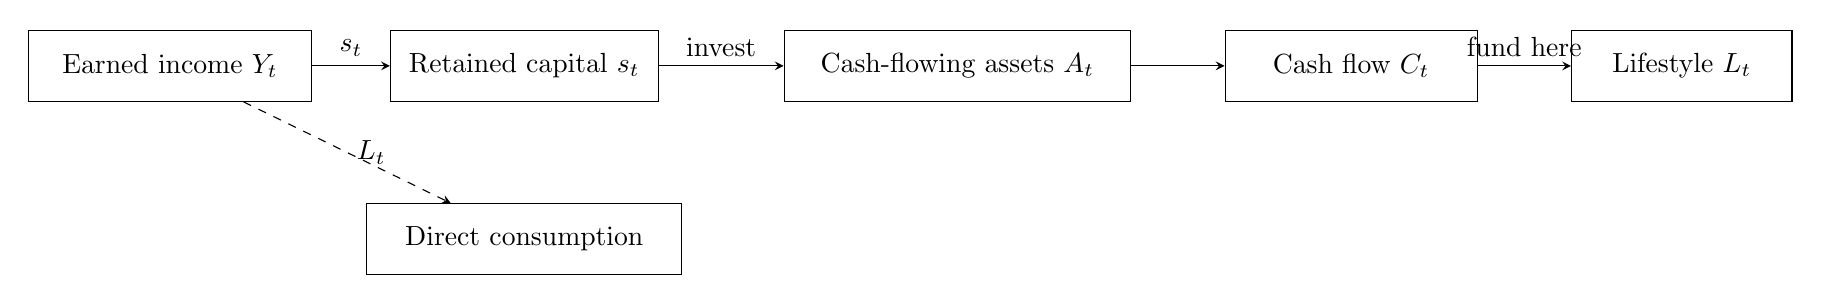
\begin{tikzpicture}[>=stealth]
\node[draw, rectangle, minimum width=3.6cm, minimum height=0.9cm] (Y) at (0,0) {Earned income \(Y_t\)};
\node[draw, rectangle, minimum width=3.4cm, minimum height=0.9cm] (S) at (4.5,0) {Retained capital \(s_t\)};
\node[draw, rectangle, minimum width=4.4cm, minimum height=0.9cm] (A) at (10.0,0) {Cash-flowing assets \(A_t\)};
\node[draw, rectangle, minimum width=3.2cm, minimum height=0.9cm] (C) at (15.0,0) {Cash flow \(C_t\)};
\node[draw, rectangle, minimum width=2.8cm, minimum height=0.9cm] (L) at (19.2,0) {Lifestyle \(L_t\)};
\node[draw, rectangle, minimum width=4.0cm, minimum height=0.9cm] (D) at (4.5,-2.2) {Direct consumption};

\draw[->] (Y) -- node[above] {\(s_t\)} (S);
\draw[->] (S) -- node[above] {invest} (A);
\draw[->] (A) -- (C);
\draw[->] (C) -- node[above] {fund here} (L);
\draw[->, dashed] (Y) -- node[right] {\(L_t\)} (D);
\end{tikzpicture}
\end{figure}

The dashed lower path is the lecture's warning. The solid upper path is its preferred mechanism.

\section{Roadmap, Time Horizon, and Strategic Pressure}

After allocation comes design. The lecture now asks how someone becomes wealthy going into 2024, and the answer changes register again. We are told to find our thing, have a blueprint, have a roadmap, and stop stumbling forward without a design. This is the moment when the lecture shifts from a money problem to a control problem.

The next move is subtle but important. We are not merely told to work hard. We are told to think far ahead. The speaker says he already knows what he is doing month over month for the next five years as he tries to move toward a still larger scale. The lecture therefore treats planning horizon as part of wealth, not as an afterthought once wealth has already been secured.

The contrast is stated in an almost aphoristic form:
\begin{align}
\text{winning posture} &= \text{macro patience} + \text{micro urgency},\\
\text{failure posture} &= \text{micro patience} + \text{macro urgency}.
\end{align}

This is not algebra in the literal sense. It is a compact statement of asymmetry. The lecture says that people typically reverse the correct pairing. They want the big outcome quickly, but they do not attack the daily moves with enough urgency. The right arrangement is the opposite: long patience at the horizon, high pressure at the daily step.

The host's recap of Eric's appearance introduces one more sharpening principle: become an expert and the best in the world at one thing. We should not flatten this into generic specialization language. In the lecture it functions as a guard against dissipation. Without one thing, one plan, and one horizon, the entrepreneur is playing checkers while the field is playing chess.

\section{Recurring Revenue, Earned Income, and Habitual Consistency}

The lecture then passes through a shorter, rougher interview whose function is not to add a polished theory but to restate the anti-fatalism theme with force. The speaker reports a best month of \$550{,}000, recalls losing \$12 million in a year and recovering from almost nothing, rejects poverty as destiny, and warns young operators not to go crazy with money because careers are finite and earnings streams can end. He uses athletes as the example: high temporary income is not a plan.

That warning prepares the way for the final, more systematic close with Wes Watson. Here the lecture returns to peak annual and monthly income, but now the host asks directly how to move from seven to eight figures. Wes answers in the language of surrounding oneself with people who think at a larger scale: people comfortable with very large monthly expenses, very expensive flights, and the use of money as a tool for larger earned income.

This produces a useful conceptual distinction. The lecture does not deny passive income, but it says that top people are still deeply attached to earned income. The recurring-revenue principle is introduced in a compressed phrase: the ``double R'' stands for recurring revenue. In the most minimal notation we may write
\begin{equation}
R_t > 0 \qquad \text{throughout the operating horizon}.
\end{equation}

Again, this is not a full revenue model. It is a way of keeping the lecture's emphasis visible: one should build a business that throws off repeatable inflow rather than relying only on sporadic wins.

The closing blueprint then moves from business design to habit design. We are told: work for it, pick the path of people one wants to resemble, do not take no for an answer, and understand social media not as distraction but as distribution. Wes's prison-to-Instagram story is especially important because it gives the lecture a long-range consistency example. He claims he saw the platform early, posted every day from prison onward, left prison with an audience, and never broke the chain. This is the lecture's last and deepest form of recurrence.

If we want a compact editorial shorthand for this final claim, we may write
\begin{equation}
H_{t+1} = H_t + h_t,
\end{equation}
where \(h_t\) is a day's packet of repeated actions: posting, training, rising early, serving others, and keeping promises. The lecture does not present this as a written formula. But it does present the directional principle clearly enough: repeated days accumulate, missed days break the structure.

The section ends with concrete daily anchors: getting up at 2:45, training at least once and sometimes several times per day, maintaining nutrition, and serving others. These details matter because they keep the lecture from dissolving into abstract mindset talk. Wealth, in the final minutes, is no longer only capital structure. It is also temporal discipline.

\section{Summary}

The lecture begins with spectacle, but it does not stay there. As we move through Miami the scattered claims slowly organize themselves into a small set of mechanisms. Patrick gives us scale and distressed entry. The e-commerce operator gives us the ladder of branding, marketing, and systems. Eric gives us the cleanest asset-allocation logic: earned income should be turned into cash-flowing appreciating assets and then into freedom. The later interviews harden the time-horizon lesson and close on recurring revenue, consistency, and habit.

So the chapter's mathematical spine is modest but real. We have a turnover ratio, a market-reset fraction, a profit-share template, an earned-income update rule, a cash-flow definition of freedom, and a contrast between the right and wrong pairing of patience and urgency. None of this was written on a board. All of it was spoken with enough force and order that we can preserve it. The lecture's final wager is that wealth is not a mysterious event. It is a sequence: enter where problems are real, build operator capacity, retain and reinvest, structure recurring inflow, and repeat the daily actions long enough for the whole machine to harden.